El impacto en la educación científica afecta la comprensión general de la astronomía.

Basándonos en el trabajo de Jordi Solbes y Rafael Palomar \cite{aprendizajeEscuelas}, concluyen que la mayoría de estudiantes en un colegio de España,
no comprenden y/o desconocen aspectos básicos de la astronomía pese a una reiterada enseñanza de la misma.

Además, confirman que un 6.2\% del alumnado sería capaz orientarse de día y noche y la sorpresa es que ningún estudiante es capaz de explicar las 
fases de la luna.

\begin{figure}[H]
    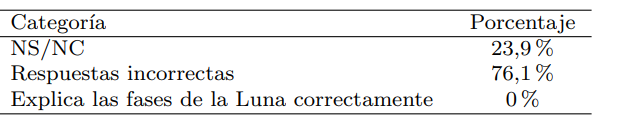
\includegraphics[scale = 0.95]{Imagenes/EspanaPrueba.png}
    \centering
    \caption{Porcentajes según puntuacion cuestionario alumnos}{Adaptado de: \cite{aprendizajeEscuelas}}
\end{figure}

Si nos basamos en el trabajo de Loyola y Ortega \cite{rabanales2021}, podemos extraer una tabla sobre una prueba realizada a alumnos en Chile sobre las fases de la luna

\begin{figure}[H]
    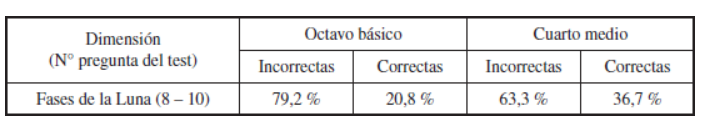
\includegraphics[scale = 0.95]{Imagenes/tablaPruebaFases.png}
    \centering
    \caption{Porcentaje de respuestas correctas e
     incorrectas en el test, sobre Fases de la Luna}{Adaptado de: \cite{rabanales2021}}
\end{figure}

Aunque no encontramos literatura que muestre datos acerca del nivel de conocimientos
en escuelas ya sea premedia y media en Panamá, sería una buena idea realizar ese estudio para tener un registro
de las nociones tendrían los estudiantes en el área de astronomía. 

Tomando en cuenta los trabajos anteriormente mencionados, podemos identifica que la forma en que se enseña la astronomía y un tema básico como el fenómeno de las fases de la luna, continúa presentándose de manera abstracta y poco
interactiva en muchos entornos educativos. Los métodos tradicionales, basados en explicaciones teóricas y representaciones estáticas, no permiten al estudiante visualizar
ni experimentar de manera dinámica la interacción entre la Tierra, la Luna y el Sol. Esta carencia de herramientas interactivas genera dificultades para comprender la esencia 
del fenómeno, reduciendo el interés y la motivación tanto de estudiantes como de docentes. 

En consecuencia, se identifica el problema principal: \textbf{la ausencia de un recurso didáctico 
basado en tecnología interactiva que facilite el aprendizaje y la divulgación de los procesos astronómicos relacionados con las fases lunares.}